%%%%%%%%%%%%%%%%%%%%%%%%%%%%%%%%%%%%%%%%%%%%%%%%%%%%%%%%%%%%%%%%%%%
%                                                                 %
%                            CHAPTER FIVE                         %
%                                                                 %
%%%%%%%%%%%%%%%%%%%%%%%%%%%%%%%%%%%%%%%%%%%%%%%%%%%%%%%%%%%%%%%%%%%

\chapter{Data Volatility} \label{Volatility}

\section{Introduction}

Capturing change counts begins to provide evidence for avoiding to use only versions to manage and describe data set change.
Figure \ref{GCMDC1} only shows the relation of the changes to each version but disconnected from time.
The changes were applied to each version, but the versions are not set to a strict schedule, meaning that many changes few changes could be applied to a version over a long or short period of time.
The change rate communicates expectations for the data consumer on the value of a data set since committing to a data set that will soon be invalidated is problematic.
The following chapter will look into data volatility, the likelihood or rate of data change, and look at how versions can hid the actual change rate of data sets.

\section{Determining Volatility}

Instead of charting the version changes in evenly wide bars, the versions are spread across time based on the time of publication to the KMS as seen in Figure \ref{GCMDPlot1}.
\begin{figure}%[b]
	\centering
	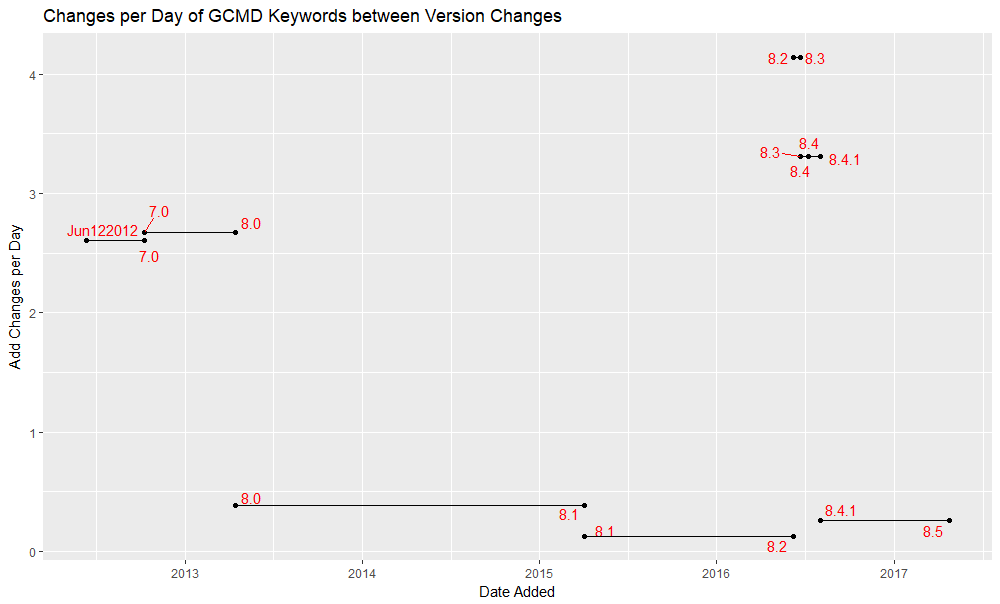
\includegraphics[scale=0.56]{figures/GCMDPlot1.png}
	\caption[Global Change Master Direcotry counts distributed over time.]{Add counts for all versions of GCMD up to 8.5 evenly distributed over the time of version validity.}
	\label{GCMDPlot1}
\end{figure}
Since each of the versions were dominated by the \textbf{Add} counts, the count is divided by the number of days between the publication of a version on the left side of the line and the release of the replacement version on the right side of the line.
The height of the line on the chart gives the steady rate of change until the release of the new version.
The area underneath the line is the total amount of change the new version introduces.
Since each version packages together all the changes into a single release, the actual change rate is unknown.

Three observable clusters appear in the time aware presentation of the versions, highlighted in Figure \ref{GCMDPlot1Cluster}.
\begin{figure}%[b]
	\centering
	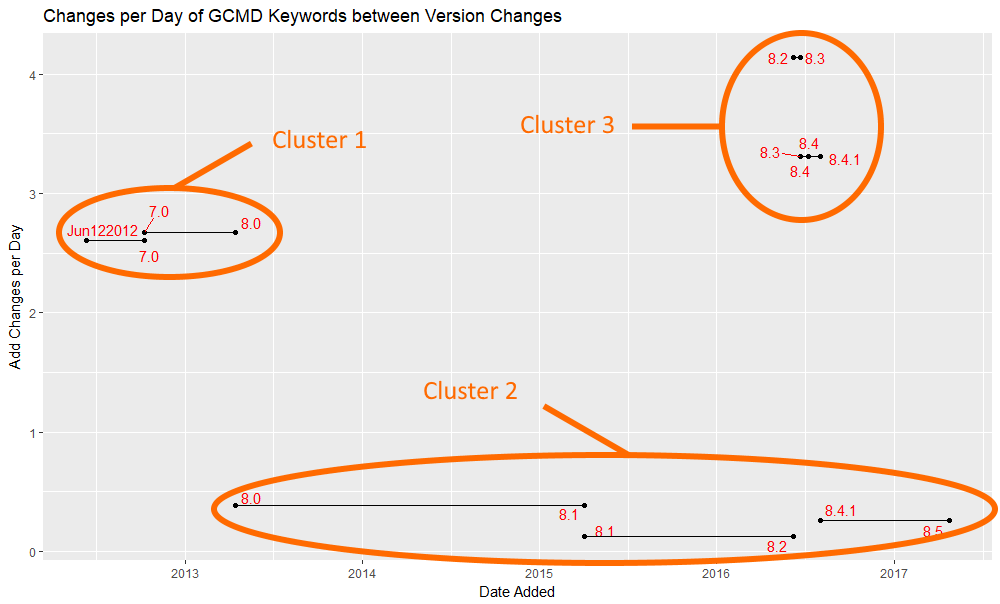
\includegraphics[scale=0.56]{figures/GCMDPlot1_Cluster.png}
	\caption[Global Change Master Directory count distributed over time with clusters marked.]{The change rate of different versions organize into three visible clusters. Cluster 2 denotes a sudden burst of version releases which is notable.}
	\label{GCMDPlot1Cluster}
\end{figure}
According to the \textit{Keyword Governance and Community Guide Document} \cite{gcmd_gov}, ``Full GCMD keywords list releases get a new major version number (e.g., 8.0). Incremental releases for updates to topics, terms, and variables get a new minor version number (e.g., 8.1).”
The statement explains the activity in Cluster 1 where there are sufficient changes to warrant a full release of the keywords.
Cluster 2 captures the change rate and duration of minor versions, except those from 8.2 to 8.4.1 which are in Cluster 3.
Cluster 3 demonstrates a flurry of activity occurring between June 7, 2016, to August 2, 2016.
Considering the previous pattern of taking at least six months between releases, three minor version releases within as many months is highly unusual.

An immediate concern is that Cluster 3 does not result from a sudden burst of activity, necessitating rapid version replacement.
An inquiry into reasoning behind the successive publication returned a statement that the government customer had requested the action.
Another way to dig into the behavior is to look into the impact assessments accompanying the versions.
Impact assessments prior to Version 8.5 are not publicly available, and only assessments for versions 8.2, 8.3, and 8.4 were received upon request.
Of the 6 requests affecting Earth Science Keywords in 8.2, published June 7, 2016, 4 were made in 2014, and the remaining 2 were made in 2015.
Version 8.3 had 8 entries in its impact assessment with 7 entries originating in 2014, and the remaining entry from 2015.
The 6 entries 8.4’s impact assessment has 5 entries from 2008 and 1 entry from 2015.
The data is collected in Table \ref{table:GCMD_old}.
\begin{table}
	\caption{Global Change Master Directory versions with old start time changes.}
	\label{table:GCMD_old}
	\centering
	\begin{tabular}{|c|c|c|c|c|}
		\hline
		Version Name&	Publish Date&	2008&	2014&	2015\\ \hline
		8.2&	June 7, 2016&	0&	4&	2\\
		8.3&	June 21, 2016&	0&	7&	1\\
		8.4&	July 7, 2016&	5&	0&	1\\
		\hline
	\end{tabular}
\end{table}


\section{Earth Observing Laboratory}

The Earth Observing Laboratory (EOL) of the National Center for Atmospheric Research (NCAR) distributes small data sets, around 10-12 files per data set, regarding lower atmospheric data beginning in 2005 \cite{EOL}.
The EOL data sets are somewhat unique in the data set size means management often does not require automation.
In mid-2014, EOL began assigning versions to stored data sets.
When receiving a new version of a data set from a researcher, the practice is to upload the entire new data set, and replace all old files.

Of the 1335 data sets maintained by EOL with versions, only 180 data sets had more than one version.  
The full distribution of version counts is in Table \ref{table:EOL_Versions}
\begin{table}
	\caption{Version Content of Earth Observing Laboratory Data Sets}
	\label{table:EOL_Versions}
	\centering
	\begin{tabular}{|c|c|}
		\hline
		Number of Versions& Number of Data Sets\\ \hline
		1&	1155\\
		2&	141\\
		3&	26\\
		4&	10\\
		5&	3\\
		Total&	1335\\
		\hline
	\end{tabular}
\end{table}
The 1155 other data sets were filtered out since change counts could not be computed for single-version collections.
Since all the files are replaced on an update and a unique file identifier like a hash sum was unavailable, file matching between versions rely on filenames to perform change mappings.
For all files that matched names across versions, the relation was classified as \textbf{Modify}.  
The approach will over-count the number of modifications, but provides an upper bound on the data set volatility in the repository.  
Each count is then normalized by the number of files in the previous version to standardize comparison between data sets regardless of data set size.  
The average for each data set is taken for each change type.

\section{EOL Versioning Behavior} \label{sec:behavior}

Given that EOL replaces the entire old data set when updating, the expected behavior of the transitions would be \textbf{Modifies} concentrating close to 1 and \textbf{Adds} and \textbf{Invalidates} distributed close to 0.
The assumption is that researchers have little reason to change the file naming scheme.
The data surprisingly indicates that data sets in EOL primarily gravitate towards \textbf{Addition} and \textbf{Invalidation} values of 1.
\textbf{Modify} counts score more close to 0 in a complete reversal of expectations.

Figure \ref{EOL_Adds} shows the distribution of \textbf{Add} scores.
\begin{figure}%[b]
	\centering
	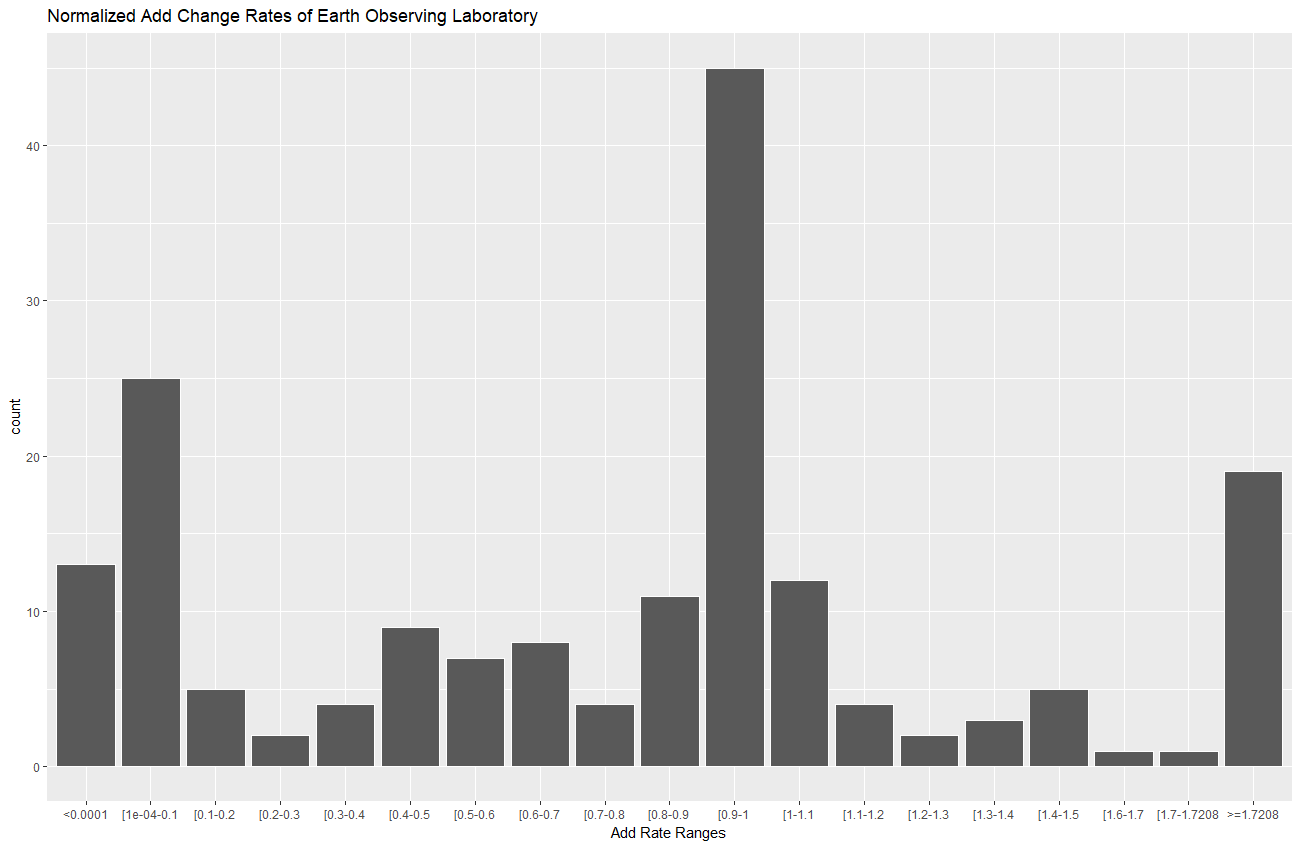
\includegraphics[scale=.43]{figures/Eol_Adds.png}
	\caption{Distribution of average normalized Add counts for each data set in Eath Observing Laboratory.}
	\label{EOL_Adds}
\end{figure}
The primary feature of the chart is the bar situated in the `[0.9-1' range, meaning that about 45 data sets add a number of files equal to the original size of the data set.
Secondary features include the bars on the far right and far left of the chart, but the bar on the right side is a collection of outliers.
In the outlier data sets, the size of the data set increased drastically compared to the behavior of other data sets managed by EOL.
Outliers are determined by collecting values above 1.5 times the interquartile range (IQR) showing in Table \ref{table:EOL_Change}.
\begin{table}
	\caption{Normalized Change Statistics}
	\label{table:EOL_Change}
	\centering
	\begin{tabular}{|c|c|c|c|}
		\hline
		Stat&	Add&	Invalidate&	Modify\\ \hline
		Mean&	0.714312707&	0.654819294&	0.345180706\\
		Std. Dev&	0.509878564&	0.420093557&	0.420093557\\
		Min&	0&	0&	0\\
		Q1&	0.28635075&	0.142857&	0\\
		Med&	0.9146635&	0.9642855&	0.0357145\\
		Q3&	1.00358625&	1&	0.857143\\
		Max&	54.25&	1&	1\\
		IQR&	0.7172355&	0.857143&	0.857143\\
		\hline
	\end{tabular}
\end{table}
A more muted distribution appears around the 0.5 mark where data sets grow more gradually.

The normalized \textbf{Invalidation} score in Figure \ref{EOL_Invs} shows a majority of data sets removing all or almost all files in the data set.
\begin{figure}%[b]
	\centering
	\includegraphics[scale=.6]{figures/Eol_Inv.png}
	\caption{Distribution of average normalized Invalidate counts for each data set in Eath Observing Laboratory.}
	\label{EOL_Invs}
\end{figure}
Coupled with the information that a quarter of the data sets added close to the original data sets' size of files suggests that the entire data set is being replaced.
\textbf{Invalidations} do not have outliers since only files within the data set can be removed.
The data is extremely biased with only 0.04 separating the median and maximum value.
From Table \ref{table:EOL_Change}, at least a quarter of values are 1.
Figure \ref{EOL_Invs} also shows a muted distrubtion around 0.5.

Figure \ref{EOL_Mods}, representing the normalized \textbf{Modify} distribution, is almost a mirror of the \textbf{Invalidation} chart.
\begin{figure}%[b]
	\centering
	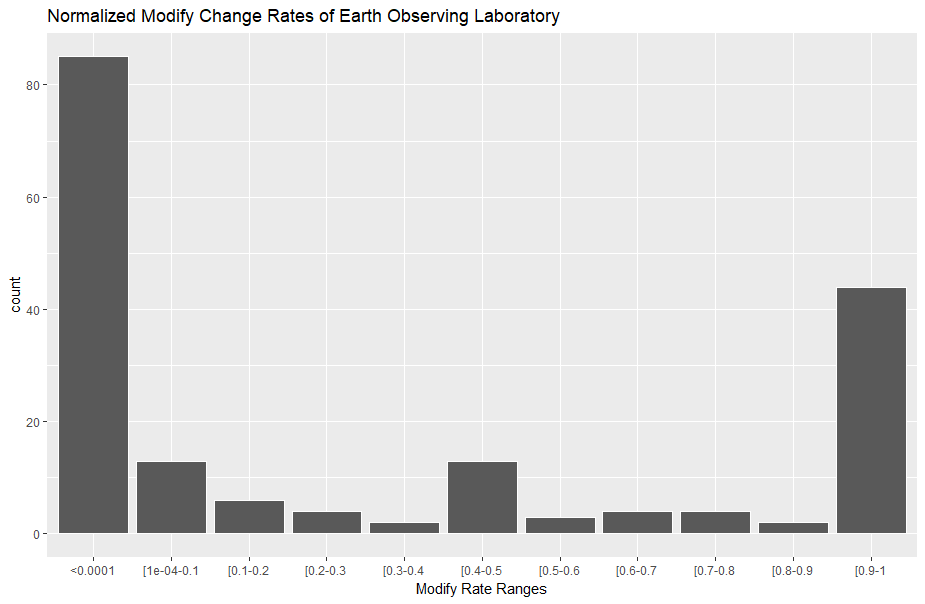
\includegraphics[scale=.6]{figures/Eol_Mod.png}
	\caption{Distribution of average normalized Modify counts of each data set in Eath Observing Laboratory.}
	\label{EOL_Mods}
\end{figure}
The right bar is specifically cut off to capture only 0s, showing that almost a majority of data sets modify 0 files, having 0 files that share names between versions.
The distribution is consistent with a practice of removing all the files in a data set and replacing the files with a new data set using different filenames.
The second feature of this graph shows around 40 data sets in which all or almost all files match across versions.
A small spike of data sets are centralized around 0.5, very much like the other normalized change graphs.

The high concentration of data sets towards 1 in \textbf{additions} and \textbf{invalidations} suggests a more complicated interaction within the data sets.
Individually, the normalized distributions do not show the connection between all three changes since the changes share a common feature, the version transition the changes describe.
Together, the AIM changes create a coordinate in three dimensional space, showing the inter-relation of the changes. 
Figure \ref{EOL_AIM} shows a scatter plot grouping unnormalized change counts for each version.
\begin{figure}%[b]
	\centering
	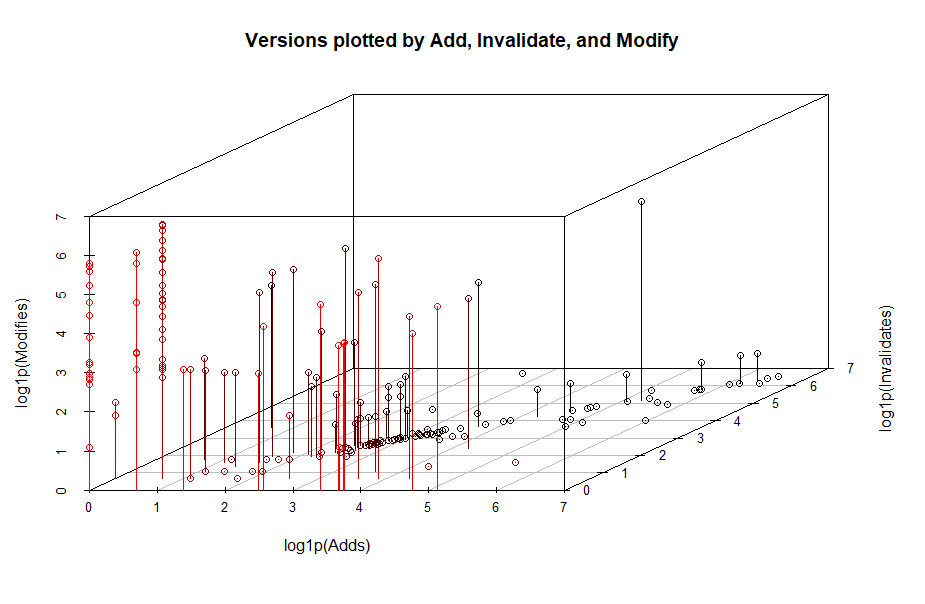
\includegraphics[scale=.6]{figures/Eol_Versions_3d.png}
	\caption{Distribution of average normalized Modify counts of each data set in Eath Observing Laboratory.}
	\label{EOL_AIM}
\end{figure}
Unlike the other charts, the size of the changes are not normalized by data set size, but the values have the log1p function applied to account for a heavy bias towards 12 and 13.
Notice the one-to-one trend between \textbf{Adds} and \textbf{Invalidates} which shows the tendency of data sets to replace every file and assign a new filename.
If the two changes did not co-occur, a normalized \textbf{Add} score of 1 would indicate that data sets tend to double in size instead.
The files are more likely to retain filenames when only a few files in a data set are being modified.

\section{Analysis}

\subsection{Impact Assessment Change Counts}

The impact assessments obtained for GCMD Version 8.2, 8.3, and 8.4 revealed that some of the changes began much earlier than the valid duration of the previous version.
Adjusting for the new duration, the change rates reduce to under 0.5, aligning with the values in Cluster 2.
The impact assessments furthermore provide change counts in the format of \textbf{Add}, \textbf{Invalidate}, and \textbf{Modify}.
In none of the cases, shown in Table \ref{table:GCMD_metric}, did the metrics completely align although Version 8.3 came close with a difference of 3.
\begin{table}
	\caption{Differences in VersOn and Impact Assessment metrics}
	\label{table:GCMD_metric}
	\centering
	\begin{tabular}{|r|r|r|r|}
		\hline
		Version & Add & Invalidate & Modify\\ \hline
		8.2(VO)&	53&	1&	26\\
		-8.2(IA)&	48&	0&	4\\
		\hline
		&	\textbf{5}&	\textbf{1}&	\textbf{22}\\
		\hline
		8.3(VO)&	58&	0&	13\\
		-8.3(IA)&	58&	0&	10\\
		\hline
		&	\textbf{0}&	\textbf{0}&	\textbf{3}\\
		\hline
		8.4(VO)&	53&	0&	1\\
		-8.4(IA)&	66&	0&	5\\
		\hline
		&	\textbf{-13}&	\textbf{0}&	\textbf{-4}\\
		\hline
		8.5(VO)&	68&	2&	22\\
		-8.5(IA)&	55&	0&	30\\
		\hline
		&	\textbf{13}&	\textbf{2}&	\textbf{-8}\\						
		\hline
	\end{tabular}
\end{table}
VersOn does not consistently overestimate or underestimate across the versions, but the assessments most consistently align on \textbf{Invalidations} which make up very few of the changes.

A investigation into the specific differences in Version 8.3 revealed that the term ``Saline Lake" does not appear in the change log, but ``Leaf Area Index (LAI)" appears twice.
LAI appears twice because it has two unique identifiers.
Six terms appeared in the change log as \textbf{Modifications} but missed three terms from the impact assessment.
The primary driver between the differences lies in impact assessments being sourced from community requests.
The focus of the change analysis becomes arranged around the preferred label rather than the unique identifier used to implement the keyword.
Impact assessments capture changes that modify a keyword's label and that doesn't change the keyword's place in the taxonomy as a result.
The change log uses a keyword's unique identifier and its placement in the taxonomy to determine changes to the structure.
The difference in metrics collection once again illustrates the producer/consumer dynamic in data version management as well as the need for clear versioning practices.
While the comparison between the two counts would be invalid due to differences in practice, a valid comparison could be constructed using the unique identifier to align entries and just the preferred label to determine if the keywords differ.

\subsection{Hidden Volatility}

To determine if the actual change rate is being obscured by the version publication rate, the duration of each version must be calculated.
Since only one version is published at the end of that duration, simply taking the inverse of the duration will give the version publication rate.
The change counts are then multiplied by the version publication rate for each version to acquire the change rate for each version.
Because the change counts are often the size of the data sets, as shown in Figure \ref{EOL_AIM}, the means must be adjusted to align with the version publication rate mean in order to perform the Kolmogorov-Smirnov test.
The test will determine the likelihood that the change distribution comes from the same distribution that produced the version publication rates.

Each version of a data set stored in EOL is assigned three different times, ``version publish time," ``version creation time," and ``version modification time." 
Version publish time indicates the time the version was made available to the public, usually the data set was added to the database.  
Version creation time denotes the moment at which a version designation was given to the collection of files, beginning in mid-2014 when the versioning system was implemented.  
Version modification time indicates the time at which the version metadata was changed.  
Using version publish time most closely resembles the duration of version validity, and the following computations use version publish time.

The duration is calculated by taking the publish time of the next version and subtracting the publish time of the current version.
Some of the durations needed to be filtered out to provide valid results.  
Due to a few coding errors in time assignments, 7 versions had to be removed because the durations were negative.  
Duration is measured in days, and the rate of version publication is determined by taking the inverse of the duration, giving versions per day.  
To acquire the AIM change rates, the changes are divided by the associated duration for each version, returning change per day.  
Since the change rates are biased towards at 0, the log of the rates are taken to give the values a more normal distribution.  
Values where an AIM change is 0 had to be removed in order to properly apply the log function.  
The size of each distribution can be found in Table \ref{table:Eol_KS}.
\begin{table}
	\caption{Summary of Kolmogorov-Smirnov Test results for Earth Observing Laboratory.}
	\label{table:Eol_KS}
	\centering
	\begin{tabular}{|c|c|c|c|c|}
		\hline
		&	Add&	Invalidate&	Modify&	Versions\\ \hline
		Length&	205&	192&	114&	227\\
		D-Value&	0.12919&	0.14464&	0.19727&	NA\\
		p-Value&	0.05487&	0.02575&	0.005443&	NA\\
		\hline
	\end{tabular}
\end{table}

Since the durations are log-normally distributed, concentrated close to 0, the log of the durations are taken to normalize the data.  
The log function is also applied to the AIM changes after the division by the duration.  
The inverse of the log of the duration is taken to acquire the rate of version release.
From Figure \ref{EOL_Add_Ver} and Figure \ref{EOL_Inv_Ver}, the change distributions, in red and green respectively, are translated a few points to the right slightly.
\begin{figure}%[b]
	\centering
	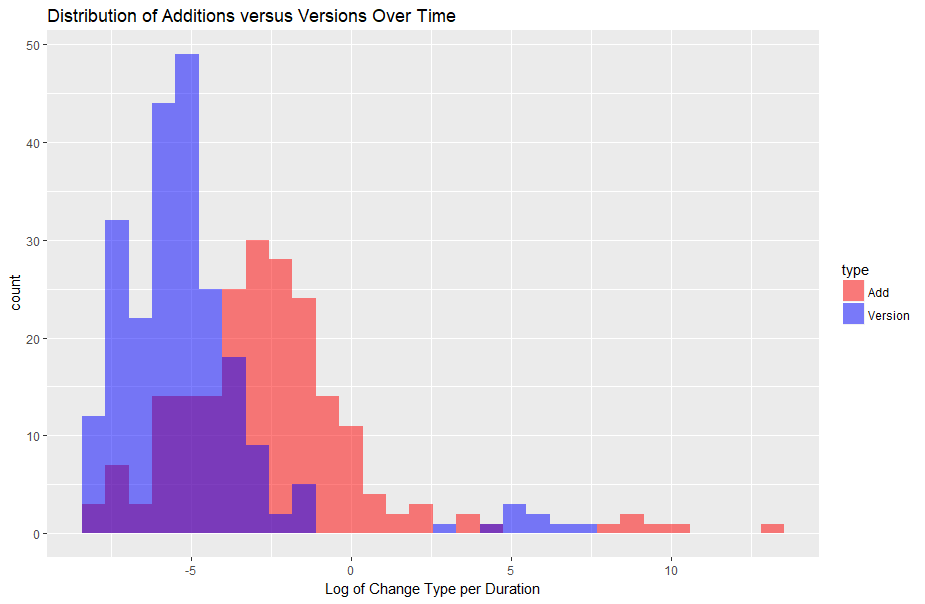
\includegraphics[scale=.6]{figures/Eol_Add_Ver_Rate.png}
	\caption{Distribution of average normalized Modify counts of each data set in Eath Observing Laboratory.}
	\label{EOL_Add_Ver}
\end{figure}
\begin{figure}%[b]
	\centering
	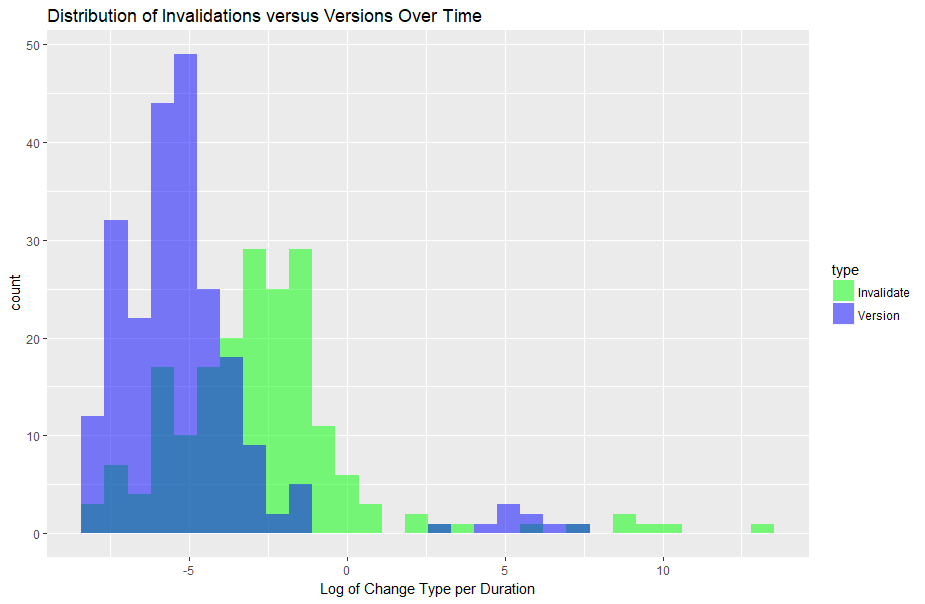
\includegraphics[scale=.6]{figures/Eol_Inv_Ver_Rate.png}
	\caption{Distribution of average normalized Modify counts of each data set in Eath Observing Laboratory.}
	\label{EOL_Inv_Ver}
\end{figure}
Because the means do not not coincide well enough, the distributions must be re-aligned at the version publication rate's mean value.
As noted in Section \ref{sec:behavior}, almost half of the versions have 0 \textbf{Modifications}, meaning that the values must be filtered out.
The resulting graph for comparison in Figure \ref{EOL_Mod_Ver} shows a more flattened \textbf{Modify} distribution.
\begin{figure}%[b]
	\centering
	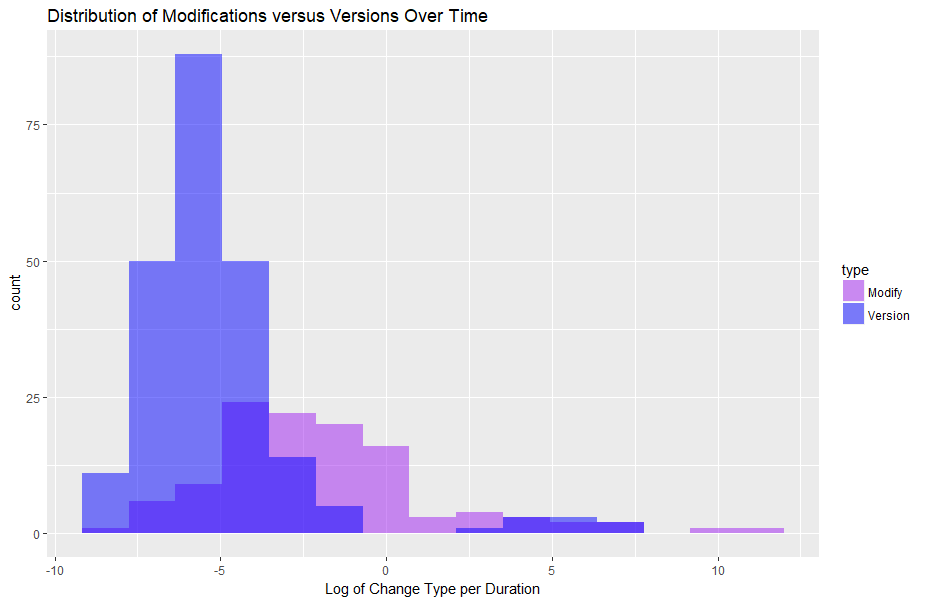
\includegraphics[scale=.6]{figures/Eol_Mod_Ver_Rate.png}
	\caption{Distribution of average normalized Modify counts of each data set in Eath Observing Laboratory.}
	\label{EOL_Mod_Ver}
\end{figure}

The Kolomogorov-Smirnov Test was used to determine if the \textbf{Adds}, \textbf{Invalidates}, or \textbf{Modifies} follow a distribution the same as the version publication distribution as the null hypothesis.  
Table \ref{table:Eol_KS} shows that the distribution of \textbf{Adds} is statistically significant with 90\% confidence while \textbf{Invalidates} and \textbf{Modifies} can reject the null hypothesis with at least 95\% confidence.
The analysis demonstrates that there is strong evidence version publications do not accurately reflect the actual change rate of the EOL data sets.

\section{Summary}

In Chapter \ref{Volatility}, we explored different ways in which versions hide the actual change behavior within a data system.
The GCMD keywords showed one perspective when evenly distributed, but spread across time, the versions have very different behavior.
The change rates, once re-coupled to time, show that versions can provide a misleading view of how changes apply to a data set.
Versions package together changes that can originate from times prior to the previous version, disrupting the assumed relationship between consecutive versions.
GCMD also breaks assumptions when the impact assessments use different metrics to determine a data set change, reinforcing the concept that perspective and context play a major role in versioning methodology.
Using only version names, Earth Observing Laboratory data is distributed uniformly by single versions, but \ref{EOL_AIM} shows a more vibrant behavior in the data sets.
The chart revealed trends in file naming and replacement.
The data sets also demonstrated that AIM changes behave significantly differently than the behavior versions reveal.